\documentclass[conference,onecolumn]{IEEEtran}

\usepackage[nolist]{acronym}
\usepackage[backend=bibtex]{biblatex}
\usepackage{graphicx}
\usepackage{hyperref}
\usepackage{pdfpages}
\usepackage[margin=3cm]{geometry}

\addbibresource{../master-thesis.bib}

\begin{document}

  \title{Proposal: Creating a web-based model transformation UI (with GLSP)}

  \author{\IEEEauthorblockN{Florian Weidner}
    \IEEEauthorblockA{Philipps-University Marburg, Germany\\
      Department of Mathematics and Computer Science, Software engineering group\\
      May 20, 2025\\
  }}

  \maketitle

  \IEEEpeerreviewmaketitle

  \section{Motivation and introduction}
  \label{sec:motivation}

  In software engineering, often \ac{mde} is used to increase development productivity and quality. Concepts are modeled closer to the domain so that they describe important aspects of a solution with human-friendly abstractions. The models can also be used to generate application fragments, that can be directly used as source code. In the process of \ac{mde}, many activities need to transform source models into different target models, while following a set of transformation rules. This model transformation process is based on algebraic graph transformations. A metamodel is used to model the structure and rules of the concept. The resulting transformation language can provide automatic model creation, development, and maintenance activities. \cite{transformations-modeldriven} One framework to use \ac{mde} is \ac{emf} by the Eclipse Foundation. It provides a basis for application development, using modeling and code generation facilities. Many frameworks build upon \ac{emf}, providing various \ac{mde} tools like code generators, graphical diagramming, model transformation or model validation. \cite{emf} One model transformation framework is Henshin. \cite{henshin-repo} It tries to provide model transformation capabilities with a high level of usability. \cite{henshin-usability} For metamodels it uses \ac{emf} Ecore files and for instance models \ac{emf} XMI files. The framework enables transformations on XMI instance files using a defined transformation language. It provides a graphical and textual syntax to create these transformation rules. \cite{henshin-repo} Henshin can be used as an eclipse plugin. Eclipse makes it easy to access, but especially for new users, the heavy editor makes using Henshin unintuitive.

  Therefore the goal exists to create a graphical option to use the Henshin model transformations without the overhead of the heavy eclipse editor. A web-based graphical editor would make using Henshin even more accessible and intuitive.

  \ac{glsp} is an open-source framework by the Eclipse Foundation to develop custom diagram editors for distributed web applications. \cite{glsp-repo} It can be used in Eclipse Desktop IDE, Eclipse Theia, Visual Studio Code, and embedded in any website. With these functionalities, \ac{glsp} fits to create an accessible, intuitive application to create and apply Henshin model transformations.

  \section{Project Requirements}
  \label{subsec:requirements}

  The following requirements are a list of the functional and non-functional requirements (that I came up with). The client should be integrated as an Eclipse Theia client. Additional clients can be added in the future without impacting other parts of your implementation. \cite{eclipseGLSP} The backend should be implemented with Java.

  Functional requirements:

  \begin{itemize}
  
    \item \ac{emf} XMI instance files should be displayed in a graphical editor
    \item Henshin rule files should be displayed in a graphical editor
    \item \ac{emf} Ecore metafiles should be displayed in a graphical editor
    \item The instance editor should display all rules that can be applied to the instance model.
    \item Parameters of the rules should be editable when applying a rule.
    \item After applying a rule, the instance model should be updated and displayed in the instance editor as a temporal file that can be used to apply multiple rules. The initial instance model should not be changed.
    \item The instance editor should provide editing functionality for the instance model.
    \item The Henshin rule editor should provide editing functionality for the transformation rules.
    \item The Ecore editor should provide editing functionality for the Ecore metamodel.

  \end{itemize}

  Once all functional requirements are implemented, the application should fully support a basic model transformation workflow. Its functionality should be equivalent to using the Henshin plugin within the Eclipse editor. It should be possible, that additional Henshin functionalities like State Space analysis or conflict and dependency analysis can be added in the future.


  Non-functional requirements:

  \begin{itemize}
    \item The application should be web-based and accessible via a web browser.
    \item The application should be responsive and work on different screen sizes.
    \item The application should be user-friendly and intuitive to use.
    \item The application should be performant and handle large models efficiently.
\end{itemize}

  \section{Basic architecture}
  \label{subsec:architecture}

  \ac{glsp} uses a client-server architecture. The client and server communicate via a websocket connection and JSON-RCP. The backend will be implemented in Java, which is the main programming language for \ac{emf} and especially the Henshin SDK. The \ac{glsp} backend supports integration with \ac{emf} models as the underlying source model for the diagrams. That makes the integration of Henshin easier because all files needed are based on \ac{emf}. The \textit{HenshinRessourceSet} can be loaded directly over the \ac{emf} integration of \ac{glsp} into the \textit{ModelState}. For the XMI instance files, the Henshin rule files, and the Ecore metamodel files, a mapping to the \ac{glsp} internal graphical model needs to be implemented. \cite{eclipseGLSP}

  For providing editing functionality, all commands need to be implemented as Actions and Handlers in the \ac{glsp} backend. They are manipulating the source files directly. The \ac{glsp} architecture is built that after manipulating the source model, the new state is mapped to the graphical model of \ac{glsp} again and then displayed in the client. \cite{eclipseGLSP} 

  The \ac{glsp} client is implemented in TypeScript. It uses Sprotty, an SVG-based diagramming framework, to render the diagrams.
  Different diagram languages can be defined for multible file types. For each file type, a different backend module must be registered. The ecore metamodel, the Henshin rule file and the XMI instance files should be in the same folder in a workspace. There you can open the corresponding file and EMF model should be displayed in a graphical editor.
  

  \section{Preliminary table of contents}
  The preliminary table of contents is on the full next page.

  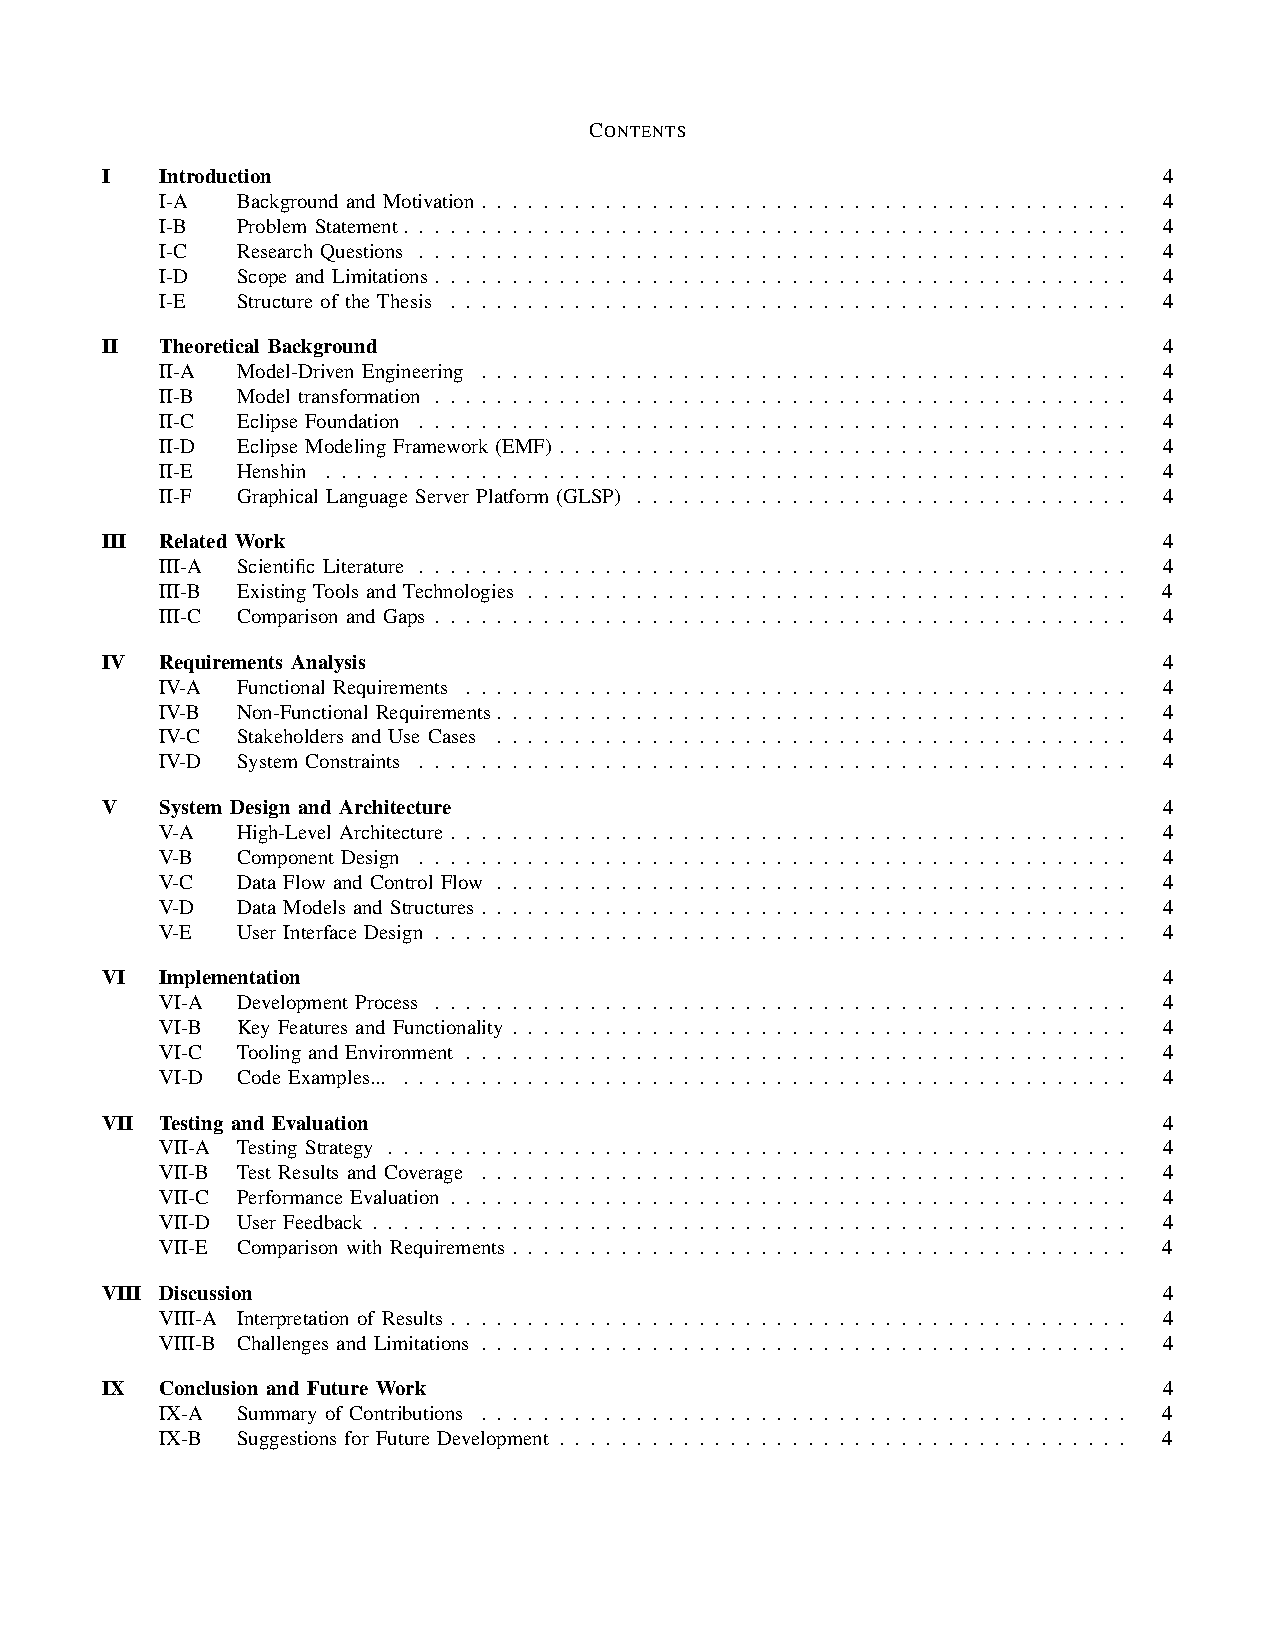
\includepdf[pages=1]{preliminary-toc.pdf}

  \section{Time schedule}
  The goal is to finish the project and the thesis at the end of August. From now on that includes 14 weeks. The three main tasks are the development of the application, writing the scientific work about the thesis, and writing the final thesis. Here is a list of the main tasks that need to be done with the estimated time needed and the planned completion date.

  \begin{table}[h!]
    \centering
    \caption{Project development tasks}
    \begin{tabular}{|p{0.5cm}|p{8cm}|l|l|}
      \hline
      \textbf{No.} & \textbf{Description} & \textbf{Estimated Time Needed} & \textbf{Planned Completion} \\
      \hline
      1 & \ac{emf} XMI instance files should be displayed in a graphical editor & 2 weeks & 24. Mai \\
      2 & The instance editor should display all rules that can be applied to the instance model. & 1 week & 31. Mai \\
      3 & Parameters of the rules should be editable when applying a rule. & 1 week & 31. Mai \\
      4 & After applying a rule, the instance model should be updated and displayed in the instance editor as a temporal file that can be used to apply multiple rules. The initial instance model should not be changed. & 1 week & 31. Mai \\
      5 & The instance editor should provide editing functionality for the instance model. & 2 weeks & 14. Juni \\
      6 & Henshin rule files should be displayed in a graphical editor & 2 weeks & 28. Juni \\
      7 & The Henshin rule editor should provide editing functionality for the transformation rules. & 1 week & 28. Juni \\
      8 & \ac{emf} Ecore metafiles should be displayed in a graphical editor & 1 week & ? \\
      9 & The Ecore editor should provide editing functionality for the Ecore metamodel. & 1 week & ? \\
      

      \hline
    \end{tabular}
  \end{table}

  \begin{table}[h!]
    \centering
    \caption{Thesis writing tasks}
    \begin{tabular}{|p{0.5cm}|p{8cm}|l|l|}
      \hline
      \textbf{No.} & \textbf{Description} & \textbf{Estimated Time Needed} & \textbf{Planned Completion} \\
      \hline
      1 & Writing basics chapter about \ac{mde} and model transformations & 1 week & 07.Juni \\
      3 & Writing basics chapter about \ac{emf} and the Eclipse Foundation & 1 week & 14.Juni \\
      4 & Writing basics chapter about Henshin and GLSP & 1 week & 21.Juni \\ 
      5 & Writing related work and existing tools & 1 week & 05.Juli \\ 
      6 & \textbf{Finishing scientific work} & 1 week & 12.Juli \\
      7 & Writing requirements chapter & 1 week & 19. Juli \\ 
      8 & Writing System Design and Architecture chapter & 2 weeks & 02. August \\ 
      9 & Writing Implementation chapter & 1 week & 09. August \\ 
      10 & Writing Testing and Evaluation 4 chapter & 1 week & 16. August \\ 
      11 & Writing Discussion chapter & 0.5 week & 23. August \\ 
      12 & Writing introduction and conclusion chapters & 0.5 week & 30. August \\ 
      \hline
    \end{tabular}
  \end{table}

  % \section{Conclusion}

  \printbibliography

\begin{acronym}
  \acro{glsp}[GLSP]{Graphical Language Server Platform}
  \acro{emf}[EMF]{Eclipse Modeling Framework}
  \acro{mde}[MDE]{Model-Driven Engineering}
\end{acronym}

\end{document}
